%\section{Experiment} \label{sec:evaluation}
%\subsection{Human Study} \label{sec:evaluation}
\section{Experimental Evaluation} \label{sec:evaluation}

In the previous case study, we showed the viability of our software transplantation approach, implemented in \autoscalpel, to generate software product lines from the existing codebase. Although the validation of the approach is based on empirical evidence, it  is  still important to test its efficiency by comparing it with other tools used to product line migration. Unfortunately, tool support for the reengineering process is limited, in general, they give support for specific activities, such as feature location, refactoring or quality assurance~\cite{Assuncao2017,Kruger2020}. To the best of our knowledge, there is currently no comparable tool that manages to transplant features from distinct donors systems written in C to generate a product line, remaining to us analysing it concerning to human effort. Thus, we conducted an experiment based on Wohlin et al.~\cite{Wohlin2012}, that reflects a real-world process of product line migration from existing codebases ~\cite{Krueger2002}. In this section, we state our research objectives and describe in detail the experimental setting.

\subsection{Goal}
The goal of this experiment is to analyse the effectiveness and efficiency of our approach compared with the manual process of generating a product line from existing systems, performed by SPL  experts. In accordance with the guidelines for reporting software engineering experiments presented in ~\cite{Wohlin2012b}, we have framed our research objectives using the Goal Question Metric (GQM) method suggested by Basili~\cite{Basili1994}. Our goal is to:

\textbf{Analyse} of a software transplantation approach to derive product variants 
\textbf{for the purpose of} comparison 
\textbf{with respect to} effectiveness and efficiency 
\textbf{from the point of view of} the researcher
\textbf{in the context of} an SPL project of product line migration from real-world systems.

\subsection{Research Questions}

In order to achieve the stated goal, we defined two quantitative questions. These are related to the data collected during the period that the experiment was executed. The questions are described as follows:

\textbf{RQ1.} \emph{What is the accuracy of the proposed approach for automated migration of target features to a product line?} In this respect, we would like to understand how accurate our approach is when automatically transferring all required code so that the target feature can run in an emergent product line compared to the manual process.

\textbf{RQ2.} \emph{How much feature migration time can be gained using \autoscalpel compared to the manual process?} With this question, we evaluate the time spent by SPL experts to \emph{extract}, \emph{adapt} and \emph{merge} features to derive new product variants in comparison with the same process using \autoscalpel. 

\subsection{Metrics}
With the objective to answer the previous questions, we defined the metrics that must be computed. For each question, it was defined one metric. These are described as follow:

\textbf{M1.} For the first question, the accuracy of our approach is computed by verifying if \autoscalpel successfully migrated new functionalities to a product line and it passed in all the regression, augmented regression and acceptance test suites. Together, these our test suites check whether or not the output of the transplanted feature is correct with respect 


%[Type Migration in Ultra-Large-Scale Codebases] For this corpus, we provide T2R with TRANSFORMATION SPECIFICATIONS to migrate seven generic Functional Inter- faces to 35 specialized alternatives. We use this corpus to assess the accuracy and usefulness of our approach (i.e., RQ1 and RQ2). Although

%Using the RefactoringMiner API, we obtain the pairs of program elements (i.e., type, method and field declarations), which have been matched between the currently analyzed commit and its parent in the directed acyclic graph that models the commit history of git-based version control repositories. The pairs of matched program elements may have identical signatures (e.g., a pair of methods with identical names, pa- rameter and return types), or may have different signatures due to refactoring operations (e.g., RENAME METHOD, CHANGE PARAMETER TYPE, ADD/DELETE PARAMETER). Java annotations are used in three different form

%Analysing each feature code successful transfered by the subjects to extract a set of common  applications that produces the delta between the commits.

%For the first question, the accuracy of our approach is computed by verifying if \autoscalpel successfully migrating new functionalities to the product line and it passed in all the regression, augmented regression and acceptance test suites. Second, analysis if the code that was automatically transplanted to the host environment is one of the selected by the SPL experts. To be more precise, if we run our approach to automatically assign a set of 100 code lines and, as a result, 70 of these code lines were correctly selected by the SPL experts, then the approach has an accuracy of 70\%. It is important to observe that different code lines can be eventually selected by different experts; however, for the purpose of the metric M1, the transplanted feature must pass at the test suite. 

%We study how frequently developers change test annotations. To provide some comparative statistics, we show the prevalence of test annotation changes compared to common source code transformations (i.e., renames and type changes) at the same program element level (i.e., class, method and field declaration). In particular, we compare test annotation changes at the method level with Rename Method and Change Return Type, at field level with Rename Field and Change Field Type, and at the class level with Rename Class. Such a comparison is attainable because all compared changes are performed on the same kind of program elements. We

%T2R generated 130 patches, out of which 126 compiled and passed the tests successfully with an overall precision of 97%.
 
\textbf{M2.} For the second question, it is simply tracked down the time that is spent with the activities to transfer the target features. Examples of these activities are \emph{code extraction}, \emph{adaptation}, and \emph{merging}. The time for each of these activities was individually collected.

\subsection{Instrumentation}


According to Wohlin et al.~\cite{Wohlin2012}, the instruments for an experiment are classified in objects, guidelines, and measurement. The object instruments of the experiment are two donor systems: \emph{NEATVI}\footnote{https://github.com/aligrudi/neatvi}, vi/ex editor for editing bidirectional UTF-8 text and \emph{Mytar}\footnote{https://github.com/spektom/mytar}, an archive manager besides another version of \emph{NEATVI} used as product base are used in this experiment. 

Manually inspecting the code to transfer a feature to a product line is hard, slow, and possibly a tedious work~\cite{Mahmood2021}. Thus, we chose to select small codebases to avoid participant's tired, in another way, it would the experiment would require too much time of execution. 

Table~\ref{tab:instrumentation} gives more details about the object instruments used in this experiment. These objects were available to download together with a script to automatic setup of the environment.  

%%%%We assume that inspecting the code to transfer a feature to a product line is hard, slow, and possibly a tedious work. Thus, we preferred this way to avoid participant's tired, in another way, it would require too much time of execution. These objects were available to download together with a script to automatic setup of the environment. 

%%According to Wohlin et al.~\cite{Wohlin2012}, the instruments for an experiment are classified in objects, guidelines, and measurement. The object instruments of the experiment are two donor systems: \emph{NEATVI}\footnote{https://github.com/aligrudi/neatvi}, vi/ex editor for editing bidirectional UTF-8 text with 7,114 LoC and \emph{Mytar}\footnote{https://github.com/spektom/mytar}, an archive manager with 1,046 LoC besides a host product base generated from \emph{NEATVI} Small systems are used in this experiment in place of the systems presented in last study. We assume that inspecting the code to transfer a feature to a product line is hard, slow, and possibly a tedious work. Thus, we preferred this way to avoid participant's tired, in another way, it would require too much time of execution. These objects were available to download together with a script to automatic setup of the environment. 

%\begin{table}[t]
%\centering \small
%	\caption{Experiment Design}
%	\label{tab:experiment_design}
%	\begin{tabular}{lll}  \\\hline
%		  & \multicolumn{2}{c}{Instrumentation} \\ 	\cline{2-3}
%		\multicolumn{1}{c}{Scenarios} & \multicolumn{1}{c}{Donor} & \multicolumn{1}{c}{Host}        \\\hline
%		I    & MYTAR & Product base  \\
%		II   & NEATVI & Product base \\\hline
%	\end{tabular}
%\end{table}


\begin{table}[t]
	\caption{Experiment instrumentation}
	\label{tab:instrumentation}
    \begin{adjustbox}{width=\columnwidth,center}
    	\begin{tabular}{l|lr|lr|lr} \hline
    		\multicolumn{1}{c}{Scenario} & \multicolumn{1}{|c}{Donors} & \multicolumn{1}{c|}{LoC}   & \multicolumn{1}{c}{Target features}       & \multicolumn{1}{c|}{LoC}  & \multicolumn{1}{c}{Host}& \multicolumn{1}{c}{LoC} \\\hline
    		I       & NEATVI & 5,276 & $\texttt{DIR\_INIT}$  & 239&\multirow{2}{*}{Product base}&\multirow{2}{*}{5,285} \\
    		II      & Mytar  & 1,046 & $\texttt{WRITE\_ARCHIVE}$ & 170&& \\\hline
    	\end{tabular}
    \end{adjustbox}
\end{table}

We recruited 20 SPL experts for the experiment that were allocated in two different groups.  We chose to allow participants to use their own work environment by avoiding adaptation bias to a strange environment with the use of unknown tools.

%%These objects were available in a cloud machine setup unpacifically to the experiment execution.

%%The MYTAR is a simple archive utility with a set of features to manager files. Although this system has only 197 LOC, it is hard to adapt one of its features to run in a product base created from a text editor.

Given this experiment involves subjects guidelines were needed to guide the participants in the experiment. It includes a process description and systems documentation. In addition to the guidelines, we provided a soft training on re-engineering to SPL and clone-and-one by assure that all participants have the same idea about the experiment objective.

For the measurement instruments, we used time sheets to track down the effort spent with the necessary activities to transfer features from existing codebase to a product base, as previously mentioned. In addition to the time sheets, we applied two forms used to collect information about the experience of subjects is shown in Table~\ref{tab:participants} and a post-survey used to better understand participants difficulties.  Further details on the operationalisation and instrumentation of this construct is presented later in the paper. 

\subsection{Hypotheses}

\textbf{Null hypothesis.} Our null hypothesis determines that there is no benefit of using the \FOUNDRY. That is, our approach cannot transplant features to generate product variants with better accuracy than manual process or the payoff is not worth. The null hypothesis is specified as follows:

\footnotesize\begin{center}H\textsubscript{0}: $\mu$(accuracy with our approach) $<=$ $\mu$(accuracy with manual process)

$\mu$(payoff with our approach) $<=$ $\mu$(payoff with with manual process)
\end{center}

\normalsize\textbf{Alternative hypothesis.} The alternative hypothesis of this experiment determines that our approach is a better option than manual approaches. That is, the proposed approach has higher accuracy and payoff. The alternative hypothesis is specified as follows:

\footnotesize\begin{center}H\textsubscript{1}: $\mu$(accuracy with our approach) $>$ $\mu$(accuracy with manual approaches)

$\mu$(payoff with our approach) $>$ $\mu$(payoff with manual approaches)
\end{center}

%\subsection{Variables}

%\normalsize\textbf{Independent variables.} There are two independent variables in this experiment, which are the approach being tested and the scenarios; we are comparing the approach proposed in this paper against another approach based on manual process. 

\normalsize\subsection{Experiment design}

We answer our research questions by simulating a real reengineering process where two features must be transferred to a product line built over a product base. The experiment design was inspired by documented real product-line migration scenarios~\cite{Laguna2013, Assuncao2017}. In the scenario I, we composed a group of 10 SPL experts where each one of them had to manually transfer all portions of code that implement the feature $\texttt{dir\_init}$ from the \emph{NEATVI} to the product base. In scenario II, another group of 10 SPL experts tried to insert the feature $\texttt{write\_archive}$ from \emph{MYTAR} into the emergent product line. In both cases, we use a reduced version of \emph{NEATVI} as the product base.
%%We answer our research questions by simulating a real reengineering process where two features must be transferred to a product line build over a product base. The experiment design was inspired by documented real product-line migration scenarios~\cite{Assuncao2017}, [39]. In the scenario I, we composed a group of 10 SPL experts where each one of them has to manually transfer all portion of code that implement the feature $\texttt{dir\_init}$ ($\sim$239 LoC) from the \emph{NEATVI} to the product base. In the scenario II, another group of 10 SPL experts tried to insert the feature $\texttt{write\_archive}$ ($\sim$170 LoC) from \emph{MYTAR} into the emergent product line. In both cases, we use a reduced version of \emph{NEATVI} as the product base (host). 
Together, these scenarios inset two new variants to our product base. The idea is to use each scenario to represent a real-context of re-engineering to SPL where systems variants came from both similar (scenario I) as distinct codebases (an archive manager providing features to a text editor's product line - scenario II) as Figure~\ref{fig:experiment_design} shows.

\begin{figure}[t]
	\centering 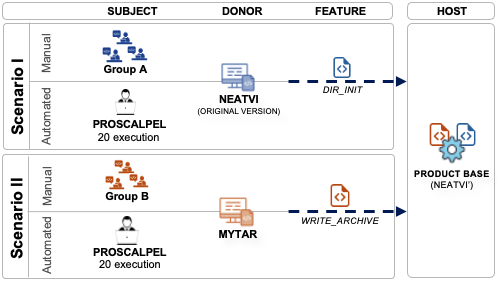
\includegraphics[width=9cm]{images/experiment_design7.png}
	\centering 
	\caption{Experiment design: one factor with two treatment applied in two re-engineering scenarios.}
	\label{fig:experiment_design}
\end{figure} 

%%%%The same process was automatically performed, following \FOUNDRY approach supported by \autoscalpel. To achieve the time and accuracy of \autoscalpel, we computed the average runtime of 20 runs transplanting a new feature variant to the product base for each scenario. Then, we report the number of \autoscalpel runs in which all test cases passed in the successful running.  


%For each run, we evaluate the degree to which the transplantation was successful by applying the same test cases and test suites used to evaluate the resulting product line generated by the participants.
 
%%%The other instrument is the system size; small features are used in this experiment in place of the features presented in last study. We assume that inspecting the code to transfer a feature to a product line is hard, slow, and possibly a tedious work. Thus, we preferred this way to avoid participant's tired, in another way, it would require too much time of execution. Further details on the operationalisation and instrumentation of this construct is presented later in the paper.
%%As we know, preparing a experiment with a manual processo of product line generating considering large code bases would be too difficult and slow process for an in-lab study. Thus, we opted by use small systems as donor systems, since it has been a scenario when our automated approach could not prove its real gains.

%%%As we know, comparing our automated approach with a manual ones as baseline considering large code bases would be too difficult and slow for an in-lab study. Thus, we opted by use small systems as donor systems, since it has been a scenario when our automated approach could not prove its real gains.

%%%As we know, preparing a experiment with a manual process of product line generating considering large code bases would be too difficult and slow process for an in-lab study. Thus, we opted by use small systems as donor systems, since it has been a scenario when our automated approach could not prove its real gains.
%%We identified the \emph{write\_archive} feature from MYTAR and \emph{dir\_init} feature from NEATVI for transplantation. 

%%Aiming to assess \FOUNDRY with respect to human effort, we conducted an experiment based on Wohlin et al.~\cite{Wohlin2012}, that reflects a real-world process of feature reuse. 
%%The design \emph{one factor with two treatments}~\cite{Wohlin2012} was used in each scenario, in which we compare the two treatments in relation to each other. The factor is the type of the approach used. For the first treatment, we tested the manual approach performed by the subjects. For the second, we tested the approach proposed in this work. For both treatments, the data used in the tests were the same, so as to avoid possible bias. 

%%%We computed the accuracy of our approaches and the time needed for transferring features to the product base in comparison with the subjects results.
%%The experiment design is showed in Figure~\ref{fig:experiment_design}.

The way used to perform the feature transferring process during the experiment represents an independent variable with two levels, manual and automated. We also distinguish participants related to the instrumentation they use: a group A, executing on scenario I and a group B, executing the scenario II. 

In this experiment, the dependent variables are the accuracy product line generation process and the payoff for using or not our approach. That is, to analyze the accuracy of the approach (RQ1), we evaluate the degree to which a transplant was successful for generating a product line. To analyze the performance of the approach (RQ2), we measured the time spent by participants to extract, adapt and merge one feature from each donor system. 

%%For each scenario, we repeat each run 20 times. Then, we report the number of \autoscalpel runs in which all test cases passed in the successful running.  

%%%%Thus, our test cases check whether or not the output of the feature is correct with respect to the original donor systems, rather than just checking the exit code.




%We proposed the extraction of one feature from each system by each group. The feature transplanted in the first scenario (group) must be small than the second one, given the limitation of the participant's time and effort required to adapt the feature to be reused in a distinct codebase. The pilot served to align them.
%We also distinguish participants related to the donor systems they use: MYTAR and NEATVI systems.



%We measured the average time spent on feature transplantation using \autoscalpel 20 times. 
%We also computed the manual effort of the participants to transfer these some feature in a product base. 


%%While participants are running the experiment, we ask them to verbalize their thoughts informing us which support strategies were being used for each stage of the features transfer process. (Protocol to think aloud [11]). When necessary, we also ask why they are performing a specific activity. The think-aloud protocol allowed us to capture data strategies and performance data simultaneously, instead of waiting until the experiments finishes to take these data. In addition, we provide an activity and time registration worksheet. We run the experiment for one participant at a time.

\subsection{Pilot Study}

Before the simulation process, we conducted two pilot studies with 6 graduate students. We used the pilot study results to determine the amount of time needed to execute our tasks and the suitable size of features. This allowed us to estimate and plan the number of participants we needed in the main study. 

The pilot study also allowed us to assess whether the participants could properly understand the subject systems and the tasks they should perform. We do not consider the results of the pilot in our analysis.

\subsection{Participants}

After the pilot, we recruited 20 participants (excluding pi-lots): 2 undergrads (Un), 9 masters (M), 7 PhD. (PhD), and 2Post-Ph.D. (Post-PhD). Most of them have more than 5 years of SPL experience and 10 years of software development. The participants are from ten different universities (from U1to U10) and the analysts/developers work in four different companies (C1, C2, C3, C4 and C5). To recruit them, we sent emails to professors in two universities, from different software reuse research groups, to suggest current and ex-members. 

Before the experiment, we asked them to answer an online survey, which we used to collect background data about their experience, mainly in software development and SPL. According to our design, we created balanced groups(A and B) of participants to each product line generation scenario based on their experience. Table~\ref{tab:participants} shows the details of the participants involved in the experiment.

\begin{table}[t]
\centering 
	\caption{\textit{Details of participants' expertise (in years) and division into groups. Group A worked on scenario I, transplanting a feature from different versions of the same donor system as the host. Group B worked on scenario II,transplanting a feature from a donor system different to the host one}}
	\label{tab:participants}
	\resizebox{7cm}{!}{%
	\begin{tabular}{clllll} \hline
%	\toprule
		Group &Part. &Degree & Inst. & \multicolumn{2}{c}{Exp. (years)}\\ \cline{5-6}
		              &         &  &   & Dev.      &  SPL     \\\hline
		A       &P1  & MSc     & U7   & [1,5)     &  [5,10)  \\%magno
    	        &P2  & Un      & C5   & [10)      &  [1,5)   \\%mateus
		        &P3  & PhD     & U4   & [10)      &  [10)    \\%jonatas
		        &P4  & MSc     & U4   & [10)      &  [1,5)   \\%marco
		        &P5  & MSc     & U4   & [10)      &  [5,10)  \\%Djan
		        &P6  & MSc     & U4   & [10)      &  [5,10)  \\%Renata
		        &P7  & PhD     & U8   & [10)      &  [10)    \\%Alcemir
		        &P8  & PhD     & U9   & [10)      &  [1,5)   \\%Tiago
	            &P9  & Pos-PhD & U10  & [10)      &  [10)    \\%Larissa
	            &P10  & PhD     & U4   & [1,5)     &  [1,5)   \\\hline%Stefani
	            
		B       &P11   & MSc     & C1   & [10)      &  [1,5)   \\%Daniel
	            &P12   & MSc     & C2   & [1,5)     &  [1,5)   \\%Rose
		        &P13   & Un      & C3   & [10)      &  [1,5)   \\%Taijara
		        &P14   & PhD     & U1   & [10)      &  [10)    \\%Michele
		        &P15   & PhD     & U2   & [10)      &  [10)    \\%Paulo
		        &P16   & PhD     & U3   & [10)      &  [5,10)  \\%Tassio 
		        &P17   & MSc     & U4   & [5,10)    &  [5,10)  \\%Rafael X
		        &P18   & MSc     & C4   & [5,10)    &  [5,10)  \\%Anna
		        &P19   & PhD     & U5   & [10)      &  [10)    \\%Iuri
		        &P20  & MSc     & U6   & [5,10)    &  [1,5)   \\\hline%Loreno 
		        
	\end{tabular}
	}
\end{table}

\subsection{Operation}

Before the participants receive their tasks, we introduced the experiment with a \emph{tutorial} about clone-and-own and reengineering of existing systems into SPL. The tutorial took 30 minutes on average.

%In general, we asked the participants to use their knowledge in C and SPL to identify, extract, adapt and deploy each feature into the same product base. 
We provided the participants with the same input as the one required for \FOUNDRY, namely: feature entry points in the donor, a set of automated unit testing, the donor’s source code, and a prepared product base with the target insertion point. Additionally, they received a few-sentence description of each feature in the target system and the system’s documentation with donor and host feature models. From those artifacts, they get domain knowledge about the systems. 
%From those artifacts, they get knowledge about the systems and how to perform the reengineering process.

The direct costs of this experiment are related solely to the time spent by the researcher with setup of the experiment itself. This involved: specifying the respective annotations for the entry point and insertion points of the features, which took approximately 13 minutes of work at the scenario I and 17 minutes at scenario II; creating the test cases, necessary to validate the target features, taking approximately 16 minutes of programming activities; preparing the product base, which took approximately 14 minutes; then, approximately 34 minutes were spent creating all documentation of donor systems including the product base feature model.

To extend the number of product base variants with a new feature transferred from the correspondent donor system, all participants had three activities based on clone\&own and the migration of cloned variants to a product line~\cite{Krueger2001,Mahmood2021}: feature \emph{extraction}, \emph{adaptation} and \emph{merging}, with descriptions and instructions provided for each task.  

Initially, the participants must identify and extract all code associated with the feature of interest to a temporary directory. Each portion of code identified as belonging to the target feature must be involved with $\texttt{\#ifdef}$ directives. For example, $\texttt{F\_DIR\_INIT}$ for the feature $\texttt{dir\_init}$. Then, the participant must rewrite extracted feature to it executes correctly in the product base environment, passing in all unit tests. To  be  more  precise, the participant has to change the feature source code to be compatible with the name space and context of its target insertion point in the product base. Finally, the participant must insert the feature code into the product base environment to validate the correctness of the feature at the emergent product line. 
%The target site in the product base was provided by us

%%If compared with approaches relying on pure machine learning algorithms, our approach needs some extra effort in order to be executed, such as: definition of the assignment rules and extraction of context information. In the context of SERPRO, although the retrieval of context information was straightforward, some extra work was necessary to insert this information in the database used by our approach. Thus, with this information in hands, we computed that 2 hours was necessary for processing and integrating the context information in the approach. In regarding to the definition of the rules, we spent about 36 hours. This involved the manual analysis and statistics of CR data, just as described in the operation. Thus, we spent a total of 38 hours for the preparation of our approach prior to the experiment’s execution.

%With respect to time needed to train the SVM algorithm, it was the same for both approaches. This was actually expected because both approaches use the same algorithm and the treatments were ran with the same dataset. Therefore, we did not consider this in our analysis since it would not change the results.

%%For each code element identified the participants must to envolve it with \#ifdef directives. Together, these scenario inset a new variants to our product base.


\subsection{Data collecting}

We have provided a task and time registration worksheet. While participants were running the experiment, we ask them to take notes of which strategies were being used for each stage of the features transfer process and why they are performing each specific task. It allowed us to capture strategies and performance data simultaneously. 

We have complemented the above setup with a post-survey. By post-survey, we could better understand participants' difficulties and meaningful differences about the manual and automated process in both scenarios. We have triangulated the data generated with the experiment with the responses we obtain from the pre and post-survey.

To establish the time for feature transplantation using our automated approach concerning manual effort, we ran \autoscalpel 20 times, and measure the average time transplanting the same feature used by the participants in each scenario. This average time was compared with the time spent by our participants on the manual re-engineering process. 

Based on our pilot study, we set a time limit of 4 hours for each manual and automated process. Another way, the result might be affected negatively by participants' boredom and tiredness. 
%The other instrument is the system size; small features are used in this experiment in place of the features presented in last study. We assume that inspecting the code to transfer a feature to a product line is hard, slow, and possibly a tedious work. Thus, we preferred this way to avoid participant's tired, in another way, it would require too much time of execution. Further details on the operationalisation and instrumentation of this construct is presented later in the paper.

%%%\subsection{Data analysis}

%%Our quantitative analysis strategy aims to build a reliable set of evidence based on the application of statistical methods. The results for each dependent variable constitute a sample, therefore, the first analysis step consists of identifying the statistical distribution for each sample through the Shapiro-Wilk~\cite{Shapiro1965} method. Its null hypothesis claims the population as normally distributed.

%%For the analysis we compared the average time of our 20 execution of \autoscalpel and the average time of the participants in the experiment. For the statistic analysis of our data, we conducted an analysis of variance using a between-subjects ANOVA. It is a parametric test for determining whether significant differences occur in an experiment containing two or more conditions. 


%CONTINUE....
%%For the qualitative analysis, we analysed the sheets and listened to the audios (post-interview) looking for commonalities and differences in the way participants execute the tasks and their perception about the manual process. We transcribed participants answers and informally generated codes to passages of the data which are relevant to understand participants difficulties and meaningful differences about the approaches used.

%%Source code. Different coding conventions used in software systems may lead to wrong conclusions. For this reason, we preprocessed the analyzed software systems by eliminating comments, empty lines, and include guards, and by applying source code pretty printing

\subsection{Results and Discussion}

We used 22 pre-existing regression test suite designed by the \emph{NEATVI} developers to assess the accuracy of \autoscalpel and answer our \textbf{RQ1}. However, they were not designed to test  \emph{NEATVI} as a product base with new variants and may not be sufficiently rigorous to find regression faults introduced by the re-engineering process. To achieve a better product line coverage, we manually augmented the host’s regression test suites with additional tests, our augmented regression suites. 

Furthermore, we implemented an acceptance test suite with 3 tests cases for evaluating the transferred feature in the scenario I and 2 for evaluating the feature in scenario II. Thus, we executed a total of 27 tests in the scenario I and 29 in scenario II, considering the acceptance tests already incorporate into the product base by the first variant inserted in scenario I. 

We summarise our results in Table~\ref{tab:transplantation_results}.  We report the status of the product base and variant inserted by the participants, the time spent and the number of passing tests for the regression augmented regression and acceptance test suites. In the first scenario, only one of the participants was not able to finish the process before the timeout. On the other hand, half of the participants were able to finish the process before achieving the timeout in the second scenario and only three of them have been able to insert the target feature without breaking the product base. 

\begin{table*}[t]
\centering 
    \caption{Experiment results comparing the time of tool over 20 repetitions with the participants:column product line status shows the generated product line status by participants and tool; column \emph{Execution Time} shows the time spent on the feature transplant by the participants and the average time of 20 run of \autoscalpel, we highlight the execution time of the participant that spent less time; column \emph{Test Suites} shows the results for each test suite; columns \emph{PASSED} report the number of passing tests; \emph{ALL} report the percent of test passed for the postoperative product line; and \emph{COV.} report statement coverage (\%) for the postoperative host and for the organ.}
	\label{tab:transplantation_results}\small
	\resizebox{18cm}{!}{%
	\begin{tabular}{llrrrrrrrrrrrrr}\\\hline
		\multicolumn{1}{c}{}      &&&    & \multicolumn{9}{c}{Test Suites}                                                                  \\
		\cline{5-9} \cline{10-13} 
		\multicolumn{1}{c}{Scenarios} & \multicolumn{1}{c}{Participants} & \multicolumn{1}{c}{ Product Line} & \multicolumn{1}{c}{Execution}& \multicolumn{3}{c}{Regression} & \multicolumn{3}{c}{Regression++.} & \multicolumn{3}{c}{Acceptance} \\
		\multicolumn{2}{c}{} & \multicolumn{1}{c}{Status} & \multicolumn{1}{c}{Time (minutes)} & \multicolumn{1}{c}{PASSED} & \multicolumn{1}{c}{ALL\%} & \multicolumn{1}{c}{COV.\%} & \multicolumn{1}{c}{PASSED} & \multicolumn{1}{c}{ALL\%} & \multicolumn{1}{c}{COV.\%} & \multicolumn{1}{c}{PASSED} & \multicolumn{1}{c}{ALL\%} & \multicolumn{1}{c}{COV.\%} \\\hline

		 \multirow{10}{*}{II} & P1 &\multicolumn{1}{l}{OK}      &\textbf{82}  & 22 &100 &-- &2 &100 &-- &3 &100 &--\\
		    & P2 &\multicolumn{1}{l}{OK}      &\textbf{88}  & 22 &100 &-- &2 &100 &-- &3 &100 &--\\
		    & P3 &\multicolumn{1}{l}{OK}      &\textbf{77}  & 22 &100 &-- &2 &100 &-- &3 &100 &--\\
		    & P4 &\multicolumn{1}{l}{OK}      &\cellcolor[gray]{.9}\textbf{68}  & 22 &100 &-- &2 &100 &-- &3 &100 &--\\
		    & P5 &\multicolumn{1}{l}{OK}      &\textbf{81}  & 22 &100 &-- &2 &-- &-- &3 &100 &--\\
		    & P6 &\multicolumn{1}{l}{Broken} & \multicolumn{1}{l}{\textbf{Timeout}}   & 0 &0  &--   &0 &0 &--   &3 &0 &--  \\
		    & P7 &\multicolumn{1}{l}{OK}      &\textbf{87}  & 22 &100 &-- &2 &100 &-- &3 &100 &--\\
		    & P8 &\multicolumn{1}{l}{OK}      &\textbf{83}  & 22 &100 &-- &2 &100 &-- &3 &100 &--\\
		    & P9 &\multicolumn{1}{l}{OK}      &\textbf{73}  & 22 &100 &-- &2 &100 &-- &3 &100 &--\\
		    & P10 &\multicolumn{1}{l}{OK}      &\textbf{113} & 22 &100 &-- &2 &100 &-- &3 &100 &--\\
		 \hline 
		 
		 \rowcolor[gray]{.9} & \textbf{\autoscalpel} &\textbf{OK in 20/20 runs} &\textbf{20} &\textbf{22} &\textbf{100} &\textbf{--} &\textbf{2} &\textbf{100} &\textbf{--} &\textbf{3} &\textbf{100} &\textbf{--}\\
		 \hline
		\multirow{10}{*}{I} & P11 &\multicolumn{1}{l}{Broken} & \multicolumn{1}{l}{\textbf{Timeout}}  & 0 &0  &--   &2 &0 &--   &0 &0 &--   \\
		 & P12 &\multicolumn{1}{l}{Broken}  & \multicolumn{1}{l}{\textbf{Timeout}} & 0 &0  &--  &2 &0 &--   &0 &0 &--   \\
		 & P13 &\multicolumn{1}{l}{Error}    &\textbf{181} & 0 &0  &--   &2 &0 &--   &0 &0 &--   \\
		 & P14  &\multicolumn{1}{l}{Broken} &\multicolumn{1}{l}{\textbf{Timeout}}   & 0 &0  &--   &2 &0 &--   &0 &0 &--   \\
		 & P15 &\multicolumn{1}{l}{Broken}  &\multicolumn{1}{l}{\textbf{Timeout}}   & 0 &0  &--   &2 &0 &--   &0 &0 &--   \\
		 & P16 &\multicolumn{1}{l}{Error}    &\textbf{114} & 0 &0  &--   &2 &0 &--   &0 &0 &--   \\
		 & P17 &\multicolumn{1}{l}{OK}       &\cellcolor[gray]{.9}\textbf{104} &25  &100 &-- &2 &100 &-- &2 &100 &-- \\
		 & P18 &\multicolumn{1}{l}{OK}       &\textbf{194} &25  &100 &-- &2 &100 &-- &2 &100 &-- \\
		 & P19 &\multicolumn{1}{l}{OK}       &\textbf{131} &25  &100 &-- &2 &100 &-- &2 &100 &-- \\
		 & P20 &\multicolumn{1}{l}{Broken} & \multicolumn{1}{l}{\textbf{Timeout}} &0   &0  &--   &2 &0 &--   &0 &0 &--   \\
		 \hline 
		 \rowcolor[gray]{.9} &\textbf{\autoscalpel} &\textbf{OK in 19/20 runs} &\textbf{27} & \textbf{25} & \textbf{100} & \textbf{--} &\textbf{2} &\textbf{2} &\textbf{--}  &\textbf{2} &\textbf{100} &\textbf{--}\\\hline

	\end{tabular}
}
\end{table*}

For each scenario, we also report the number of \autoscalpel runs in which the product derived passed in all test cases in the successful running. For each scenario, we repeat each run 20 times. The success rate was retained for both scenarios I and II, where we lost only one successful run in the timeout and the product line generated passed in all tests in all test suites.

\begin{framed}
\noindent To answer \textbf{RQ1},the results show success of  rate was retained for both scenario I and II, where we lost only one successful run in the timeout and all products derived passed in all test in all test suites.  
\end{framed}

As stated in the definition of the metric \textbf{M2} and to answer \textbf{RQ2}, we evaluate the payoff of \FOUNDRY. Figure~\ref{fig:experiment_result_time_II} graphically shows the time spent on each activity performed in re-engineering to SPL process. In summary, Group A transferred the target feature from \emph{NETVI} to the product base in 1h24 minutes on average. \autoscalpel turned out to be quicker, successfully transplanting this feature in all 20 trials, in an average of 20 minutes.

\begin{figure}[t]
	\centering 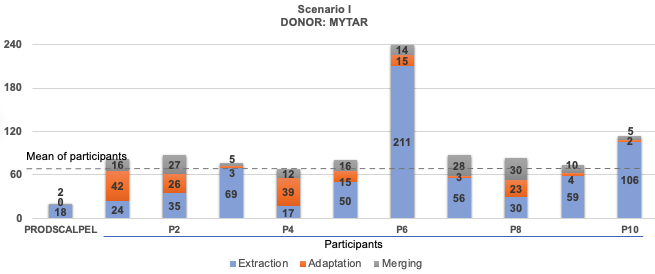
\includegraphics[width=8.5cm]{images/experiment_result-SC1-4.png}
	\label{fig:experiment_result_time_I}
\end{figure} 
\begin{figure}[t]
	\centering 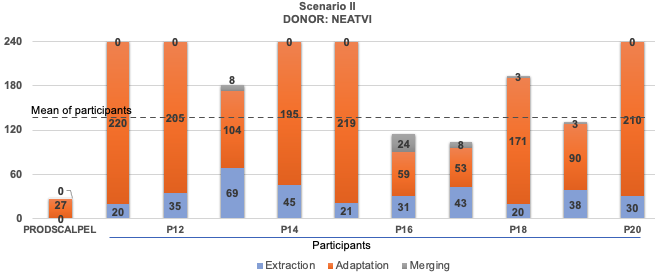
\includegraphics[width=8.5cm]{images/experiment_result-SC2-4.png}
	\centering \caption{Time (in minutes) spent by participants and \autoscalpel on performing the three stages of SPL reengineering: feature \emph{extraction}, \emph{adaption} and \emph{merging}. The graph highlight the average participants time that successful generated its target product line.} 
	\label{fig:experiment_result_time_II}
\end{figure} 

Most of the participants of Group B had not completed the product line generation process from \emph{Mytar}  within the 4 hours time limit. Considering the participants that were able to finish the process (i.e., participants \emph{P17}, \emph{P18} and \emph{P19}) and its product line passed in all test suites they spent an average of 2h23 minutes while \autoscalpel was able to complete this task in 19 of 20 trials in the timeout, taking 27 minutes on average.

\textbf{Statistic analysis of performance.} The quantitative analysis strategy from the experiment was adapted to this study because there is no comparison between scenarios since used different donors and target features. The first analysis step consists of identifying the statistical distribution for each scenario through the Shapiro-Wilk~\cite{SHAPIRO1965}, a method with the best power for a given significance~\cite{Razali2011}. Its null hypothesis claims the population is normally distributed. It determines which set of methods must be applied in the hypothesis testing and the strength of association between variables. 

Figure~\ref{fig:experiment_result_boxplot} graphically shows the time results for our two groups in comparison with \autoscalpel performance. In the scenario, I, the preliminary information provided by the box plots indicate that all samples are normally distributed (W = 0.70445, p-value = 3.129e-05). Thus, a ANOVA~\cite{Gelman2005} and Pairwise Student’s t-test analysis were conducted considering the hypothesis of the time values for \autoscalpel have statistically higher values if compared to the manual methods (p-value $<$ 2e-16). It led to the rejection of the null hypothesis for all pairs. 

In the scenario II, the normality test result showed a normal distribution with a W = 0.69378, p-value = 1.715e-06. Thus, we used ANOVA to hypothesis testing and Pairwise t-Student. Based on the ANOVA test and Pairwise t-Student, we rejected the null hypothesis (p-value $<$ 2e-16) that the distribution of the population is homogeneous.

We can concludes that \autoscalpel reduces developer effort to transfer features to a product line in both scenarios. For both simulation scenarios, there is a significant effect size between the tasks performed in a manual way and using \autoscalpel. The participants had similar performance times in scenario I, with the exception of the participants \emph{P6}. On the other hand, most of the participants of scenario I do not terminate the experiment before the 4-hour timeout. This last one is qualitatively explained by the participants in the post-survey where they exposed how 
hard is to adapt a feature to run in a strange codebase. 
 
\begin{figure}[t]
	\centering 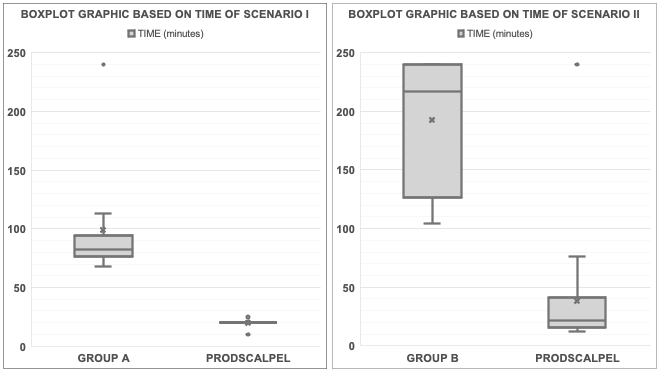
\includegraphics[width=8.9cm]{images/experiment_time_results.png}
	\centering 
	\caption{Time results grouping automated and manual in both scenarios.  Scenario I: \emph{NEATVI} - Product Base; Scenario II: \emph{Mytar} - Product base.}
	\label{fig:experiment_result_boxplot}
\end{figure} 


\begin{framed}
\noindent To answer \textbf{RQ2}, in both scenarios \autoscalpel outperformed participants with respect to the average task time. By considering the sum of time spent with both scenarios, the tool accomplished the product line generation process  by inserting two new variants in 4.8 times faster than the mean of participants were able to finish the experiment in the timeout and their resulting product line passed in all test cases.
\end{framed}

\section{Threats to Validity}

The threats to the validity of this study are mainly related to external and internal validity~\cite{Wohlin2012}. Conclusion validity issues involve the low power of the statistical analysis. The number of SPL projects can be a threat to the hypotheses not rejected in this experiment. Aiming to address it, the extension of the experiment to incorporate new donors systems is being explored, and improved results will be reported in future work. In addition, we already provide a set of heterogeneous systems, with distinct characteristics in terms of domains, amount of code lines, and numbers of features. It provides a representation on how the \autoscalpel approach behave when applied to different objects as an archive manager providing features to generate a text editors product line.

\textbf{External Validity.} The relatively small number and diversity of systems used for generating a product line pose an external threat to validity. We applied our results to small programs due to the boundaries of an in-lab study; our results may not generalize to larger programs in the wild. We tried to mitigate it by constructing possible real-world scenarios, i.e., reuse of features from unrelated codebase and variations of the same systems, both real-world systems. Additionally, given that our approach was helpful even in small programs, we argue that is likely helpful for larger systems as it is nearly impossible to incorporate new variants to a product line without a large understanding of the donor systems specifications or without specialized tool support~\cite{Assuncao2017}.

%Justyna: I don't want to draw attention to that.
%\textbf{Construct Validity.} We did not compare our tool using a real-world SPL extracted from NON-SPL as a baseline. A critical part of the validation of a tool for SPL reengineering from existing systems is to find a suitable baseline that defines a transition process between NON-SPL systems codebases to an  SPL or even a tool that performs such process with codebases written in C. Although the task without specialized tool support is too difficult and slow, it is useful as a baseline to investigate the benefits of \FOUNDRY by provide an automated solution to the process. 

\textbf{Internal Validity.} Due to time expensive nature of a human study, we had few participants. We tried to mitigate this issue by selecting participants with considerable experience in SPL projects. The other threat to the validity is the system size; small features are used in this experiment. We assume that inspecting the code to transfer a feature to a product line is hard, slow, and possibly a tedious work.  Thus, we preferred this way to avoid eventual human error as consequence of participant's tired, in another way, it would require too much time of execution. Even with a limited execution time, we were able to transplant features from donors with significant size (consisting the more than 6k LoC of our donor systems together, as shown in Table~\ref{tab:instrumentation}. We also use testing as means of validating our approach, which cannot provide a formal proof of its correctness.  We used extensive testing to mitigate this risk. Moreover, testing is a standard approach to code evaluation in real-world scenarios due to its high scalability.